\begin{figure}[h]

    \centering
    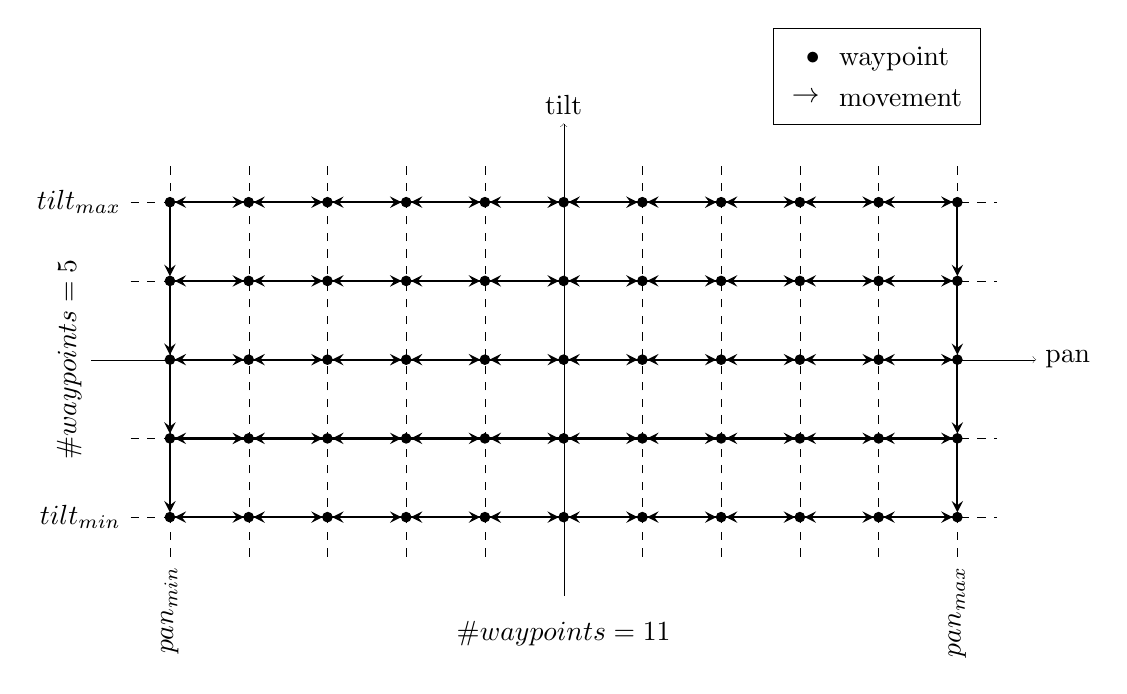
\begin{tikzpicture}

        \draw[->, ultra thin] (-6, 0) -- (6, 0) node[right] {pan};
        \draw[->, ultra thin] (0, -3) -- (0, 3) node[above] {tilt};

        \draw[step=1, ultra thin, dashed] (-5.5, -2.5) grid (5.5, 2.5);

        \foreach \x in {-5,...,5}
            \foreach \y in {-2,...,2}
                \draw[fill=black] (\x, \y) circle (0.06);
        
        \foreach \x in {-5,...,4}
            \foreach \y in {-2,...,2}
                \ifthenelse{\isodd{\y}}{
                    \draw[stealth-, shorten <=0.06cm, thick] (\x, \y) -- (\x+1, \y);  
                }{
                    \draw[-stealth, shorten >=0.06cm, thick] (\x, \y) -- (\x+1, \y);
                };

        \foreach \y in {2,...,-1}
            \ifthenelse{\isodd{\y}}{
                \draw[-stealth, shorten >=0.06cm, thick] (-5, \y) -- (-5, \y - 1);
            }{
                \draw[-stealth, shorten >=0.06cm, thick] (5, \y) -- (5, \y - 1);
            };

        
        \node[anchor=east] at (-5.5, -2) {$tilt_{min}$};
        \node[anchor=east] at (-5.5, 2) {$tilt_{max}$};
        \node[anchor=south, rotate=90] at (-6, 0) {$\#waypoints = 5$};

        \node[anchor=east, rotate=90] at (-5, -2.5) {$pan_{min}$};
        \node[anchor=east, rotate=90] at (5, -2.5) {$pan_{max}$};
        \node[anchor=north] at (0, -3.2) {$\#waypoints=11$};
            
        \matrix[draw, above left, xshift=-1.5cm, yshift=-0.5cm] at (current bounding box.north east) {
            \node[label=right:waypoint] {$\bullet$}; \\
            \node[label=right:movement] {$\rightarrow$}; \\
        };

    \end{tikzpicture}

    \caption{Waypoints and movements in the pan/tilt joint space.}

\label{figure:joint-movement}
\end{figure}
